\subsection{Specific Privacy}

In addition to the Zcash team, other public blockchains that implement private transactions include Monero \cite{website:Monero}, Dash \cite{website:Dash}, Grin \cite{website:Grin}, and more. However, these public chains lack programmability and can only be used for private asset transfers. Consequently, their ecological development lags far behind Ethereum, which has become the largest public chain in the ecosystem due to its programmability, but lacks privacy features.

Therefore, some projects have begun to explore ways to introduce privacy to Ethereum, such as the ZK-ZKRollup application zk.money \cite{website:zk.money} developed by the Aztec \cite{website:Aztec} team. However, the current zk.money product has been discontinued, mainly because it can only be applied to a single privacy transfer scenario. Given the current explosion of Defi applications, asset transfer is only one of the simplest financial scenarios, and therefore the user base is limited, while the maintenance costs continue to accrue.
\begin{figure}[!ht]
    \centering
    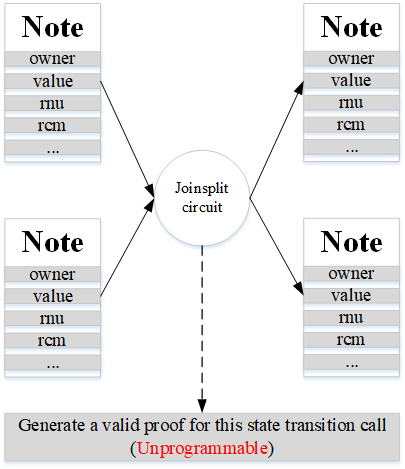
\includegraphics[width=0.4\textwidth]{Example of Specific privacy.jpg}
    \caption{Example of Specific Privacy}
    \label{fig:Example of Specific privacy}
\end{figure}

\figref{fig:Example of Specific privacy} shows the simple logic of specific privacy. Since the scene is single (most of them are privacy transfers), the value change logic corresponding to the input and output notes in Section \ref{section: sending-notes} are also fixed, generally in the form of ``A + B = C + D''. Manta Network \cite{website:Manta-network} is a public blockchain that supports user-defined token privacy transfers, and the privacy transaction 
constraint circuits of all fungible tokens can be used to reuse the above logic.

The ZK-ZKRollup application of a single scene is like the ZKRollup application of a single scene. If you want to use the asset for other scenarios, you must cross the asset to another application through a bridge, which is very unfriendly to the user experience. Therefore, just as ZKRollup needs to 
transition to ZK(E)VM, ZK-ZKRollup also needs to transition to ZK-ZKVM (Appendix \ref{section: solidity-compatibility} explains how to get solidity compatibility).
